{A right circular cone with height of 10 and base radius of 5. \label{ex_07_02_ex_18}

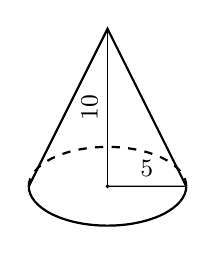
\begin{tikzpicture}[scale=.5]
\begin{scope}[xscale=2]
%\draw [thick](0,0) circle (1);
\draw [thick] (-1,0) arc (180:360:1);
\draw [thick,dashed] (1,0) arc (0:180:1);
\end{scope}

\draw [fill=black] (0,0) circle (1pt) -- node [pos=.5,above] {\small 5} (2,0);
\draw (0,0) -- node [pos=.5,rotate=90,above] {\small 10} (0,4);
\draw [thick] (-2,0) -- (0,4)-- (2,0);
\end{tikzpicture}
}
{Placing the tip of the cone at the origin such that the $x$-axis runs through the center of the circular base, we have $A(x)=\pi x^2/4$. Thus the volume is $250\pi/3$ units$^3$.
}
